\chapter{Experiments and Results}

\section{Introduction}
This chapter reports the experiments in the order the system runs them: the setup, the data actually used, model selection and tuning on 2024, the sealed test, the expected ranges, the alerts, the driver breakdown, an example of the output, and a discussion.

\section{Experimental Setup}

\subsection{Hardware Configuration}
Data preparation, the audit and the dashboard ran on a personal Windows computer. All model fitting ran on Google Colab with a CPU runtime and no accelerator, limited to two threads in the fits (Table~\ref{tab:hardware}).

\begin{table}[H]\centering\small
\caption[Hardware configuration]{Hardware configuration.}\label{tab:hardware}
\begin{tabular}{lp{8cm}}
\toprule
\textbf{Component} & \textbf{Details} \\
\midrule
Work computer & Windows 10; data conversion, audit, unit tests, local dashboard \\
Model fitting & Google Colab, CPU runtime, no GPU; two threads used by the fits \\
Storage & Google Drive folder for data, results and models; GitHub repository for code \\
\bottomrule
\end{tabular}

\end{table}

\subsection{Software Environment}
Table~\ref{tab:software} lists the tools. The Colab notebooks clone the code from GitHub at each start, so the code is not stored on Drive.

\begin{table}[H]\centering\small
\caption[Software environment]{Software environment.}\label{tab:software}
\begin{tabular}{lp{8cm}}
\toprule
\textbf{Tool} & \textbf{Use} \\
\midrule
Python 3.13 (Colab) & all stages \\
pandas, pyarrow & price panel and feature tables \\
LightGBM & main model \\
Optuna & tuning, 50 trials \\
statsforecast (AutoETS) & ETS candidate \\
scikit-learn & ridge and random forest candidates \\
PyTorch (CPU) & LSTM candidate \\
Gradio, Streamlit & dashboard in Colab and on the work computer \\
pytest & unit tests and stage acceptance checks \\
\bottomrule
\end{tabular}

\end{table}

\subsection{Implementation Details}
Six Colab notebooks run the stages in order: data and features; model selection and tuning; the sealed test; alerts and drivers; the production fit and export; and a notebook that shows the exports and downloads them. Each stage writes its results to Google Drive and records a hash of every output, so a stage that has finished is skipped on a rerun, and a dropped runtime resumes from the saved pieces. The test is guarded by a seal record that allows one scoring per committed pre-registration. A rerun after the 2025--26 test had already been scored reused the saved forecasts and the same seal, and reproduced the same numbers.

\section{Dataset Description}

\subsection{Dataset Distribution}
Table~\ref{tab:strata} shows the items by group. The model uses 54 items. For the validation year there were 43 origins from 2024-01-01 to 2024-11-24, and for the test 87 origins from January 2025 to October 2026.

\subsection{Price Change Frequency}
The share of forecasts where the price actually changed rises with the horizon (Table~\ref{tab:test}). At 1 report day ahead the price changed in 6.9\% of the cases, at 7 in 25.6\%, at 14 in 37.7\% and at 30 in 52.4\%. This is the main property of the data: at the short horizons almost every correct forecast is ``no change''.

\section{Training and Tuning Results}

\subsection{Model Selection on 2024}
No candidate beat the naive forecast on the 2024 validation origins (Table~\ref{tab:select}). ETS came closest, at 5\% worse than naive overall, LightGBM was 17\% worse, and ridge regression was worst. Because the naive forecast cannot be chosen, ETS was the nominal winner. The explanation step needs a tree model, so I kept LightGBM as the main model and logged that decision, with this table, before tuning. The model was therefore not chosen because it won the comparison, and the results below should be read with that in mind.

\begin{table}[H]\centering\small
\caption[Validation on 2024, six candidate models]{Validation on 2024, 43 origins, all four horizons. Lower is better; relative error 1.000 is a tie with ``tomorrow equals today''.}\label{tab:select}
\begin{tabular}{lrr}
\toprule
\textbf{Model} & \textbf{Error of log change} & \textbf{Relative to naive} \\
\midrule
Naive (tomorrow = today) & 0.0231 & 1.000 \\
ETS & 0.0235 & 1.053 \\
LightGBM & 0.0241 & 1.173 \\
LSTM & 0.0245 & 1.378 \\
Random forest & 0.0272 & 1.698 \\
Ridge regression & 0.0292 & 2.316 \\
\bottomrule
\end{tabular}

\par\smallskip{\footnotesize Source: \path{reports/project/tables/P5_model_selection_overall.csv}.}
\end{table}

\subsection{Tuning}
Across the 50 trials the best score on the tuning origins was 0.02478 and the median trial was 0.02486, so most settings that were not clearly bad ended up almost the same. The default setting scored 0.02592 on the tuning origins and 0.02050 on the confirmation origins; the best trial scored 0.02478 and 0.01969. The tuned model is small (Table~\ref{tab:params}). The tuning found a better setting, and it also found one that moves the forecast very little from zero.

\subsection{Learning Curve}
Over 400 trees the training error went from 0.0305 to 0.0302, and the error on a holdout of the latest 15\% of report days did not improve (0.0171 to 0.0172, Figure~\ref{fig:lc}). Adding trees gave the model nothing more to learn from these inputs.

\begin{figure}[H]
\centering
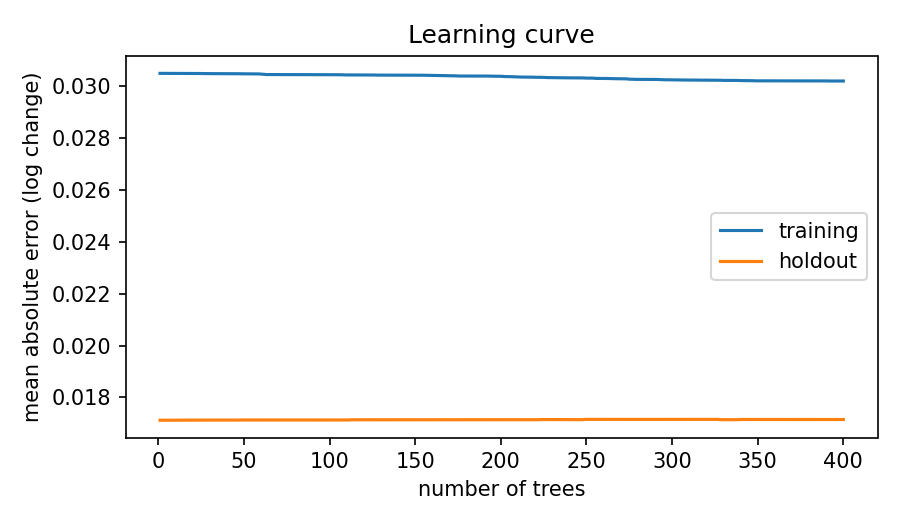
\includegraphics[width=0.7\textwidth]{F13_learning_curve.png}
\caption[Training and holdout error by number of trees]{Training and holdout error by number of trees.}\label{fig:lc}
\par\smallskip{\footnotesize Source: \path{reports/project/figures/F13}.}
\end{figure}

\section{Evaluation Results}

\subsection{Test Accuracy}
On the sealed test the model matches the naive forecast closely and does not beat it at any horizon (Table~\ref{tab:test}, Figure~\ref{fig:rel}). The geometric-mean relative error is 1.0096, 1.0013, 1.0009 and 1.0007 at horizons 1, 7, 14 and 30. At horizons 1 and 7 the model is worse by a margin that is small in size but clear in the Diebold--Mariano test ($p=0.0001$ and $0.011$); at horizons 14 and 30 there is no detectable difference ($p=0.92$ and $0.50$).

The reason is visible in the error split. Most of the error comes from days when the price moved: at horizon 7 the error is 0.0467 on days the price changed and 0.0001 on days it did not, and the price changed on 26\% of those forecasts. The model predicts almost no change, so it is nearly perfect on unchanged days and about as wrong as the naive forecast on changed ones. The coefficient of determination on the price changes is between $-0.002$ and $0.012$. Direction is right on only 15\% to 38\% of the days where the price moved, which is what a forecast of no change would give.

\begin{table}[H]\centering\small
\caption[Sealed test results by horizon]{Sealed test, January 2025 to October 2026, 87 origins. Relative error is the geometric mean over 54 items of model error divided by naive error.}\label{tab:test}
\begin{tabular}{rrrrrrr}
\toprule
\textbf{Horizon} & \textbf{Model error} & \textbf{Naive error} & \textbf{Relative error} & \textbf{Error (Tk)} & \textbf{Price changed} & \textbf{DM $p$} \\
\midrule
1 & 0.0028 & 0.0027 & 1.0096 & 3.1 & 0.069 & 0.0001 \\
7 & 0.0120 & 0.0120 & 1.0013 & 23.8 & 0.256 & 0.011 \\
14 & 0.0199 & 0.0199 & 1.0009 & 43.2 & 0.377 & 0.92 \\
30 & 0.0323 & 0.0324 & 1.0007 & 79.2 & 0.524 & 0.50 \\
\bottomrule
\end{tabular}

\par\smallskip{\footnotesize Source: \path{reports/project/tables/P7_accuracy_by_horizon.csv} and \path{P7_dm_vs_naive.csv}.}
\end{table}

\begin{figure}[H]
\centering
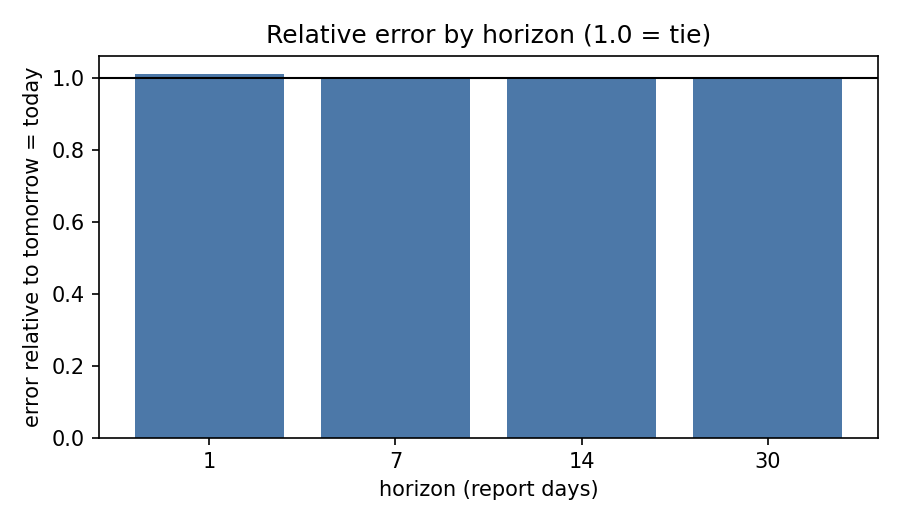
\includegraphics[width=0.7\textwidth]{F10_relative_error_by_horizon.png}
\caption[Relative error by horizon on the test]{Relative error by horizon on the test (1.0 is a tie with ``tomorrow equals today'').}\label{fig:rel}
\par\smallskip{\footnotesize Source: \path{reports/project/figures/F10}.}
\end{figure}

\subsection{Results by Item Group and Item}
Item by item the picture is the same. Out of 54 items, the model had a lower error than the naive forecast for 13 items at horizon 7, 13 at horizon 14 and 16 at horizon 30, and the ratio ranged from 0.96 to 1.03 (P7\_accuracy\_by\_item.csv). By group, the ratio was between 0.998 and 1.017 everywhere (Table~\ref{tab:group}). The only group-and-horizon cells below 1 are administered items at 30 days (0.999) and volatile perishables at 14 and 30 days (0.999 and 0.998), and these differences are far too small to count as evidence.

\begin{table}[H]\centering\small
\caption[Relative error by item group and horizon]{Relative error to the naive forecast by item group and horizon on the test (geometric mean over items).}\label{tab:group}
\begin{tabular}{lrrrr}
\toprule
\textbf{Group} & \textbf{h = 1} & \textbf{h = 7} & \textbf{h = 14} & \textbf{h = 30} \\
\midrule
Administered & 1.008 & 1.001 & 1.001 & 0.999 \\
Domestic staples & 1.017 & 1.004 & 1.002 & 1.002 \\
Imported staples & 1.003 & 1.001 & 1.001 & 1.002 \\
Non-food & 1.001 & 1.000 & 1.001 & 1.002 \\
Spices & 1.014 & 1.001 & 1.000 & 1.001 \\
Volatile perishables & 1.017 & 1.003 & 0.999 & 0.998 \\
\bottomrule
\end{tabular}

\par\smallskip{\footnotesize Source: \path{reports/project/tables/P7_accuracy_by_group.csv}.}
\end{table}

\subsection{Robustness Checks}
The two further schemes give the same answer, and the older walk-forward years are worse for the model (Table~\ref{tab:wf}). In 2023 the model was 11\% worse than naive at horizon 1 and 3\% worse at the other horizons. The sliding-window version was a little worse than the expanding window on the test.

\begin{table}[H]\centering\small
\caption[Relative error under other evaluation schemes]{Relative error to the naive forecast under the other evaluation schemes.}\label{tab:wf}
\begin{tabular}{lrrrr}
\toprule
\textbf{Scheme} & \textbf{h = 1} & \textbf{h = 7} & \textbf{h = 14} & \textbf{h = 30} \\
\midrule
Rolling origin 2025--26 (main) & 1.0096 & 1.0013 & 1.0009 & 1.0007 \\
Walk-forward 2023 & 1.1143 & 1.0294 & 1.0272 & 1.0253 \\
Walk-forward 2024 (tuning year) & 1.0343 & 1.0047 & 1.0027 & 1.0027 \\
Sliding window of 500 reports & 1.0270 & 1.0078 & 1.0077 & 1.0047 \\
\bottomrule
\end{tabular}

\par\smallskip{\footnotesize Source: \path{reports/project/tables/P7_walk_forward.csv}.}
\end{table}

\subsection{Error Analysis}
The error analysis (P7\_error\_analysis.csv) shows no difference between normal periods and the weeks around Ramadan and the Eids beyond a slightly larger error in the latter for both the model and the naive forecast (0.0126 against 0.0119 at horizon 7). The bias, meaning the mean of forecast minus actual in log terms, is close to zero (mean $-0.00008$ across origins at horizon 7, Figure~\ref{fig:bias}). The largest forecast errors are mostly for ginger in January 2025 at the 30-day horizon, with a log error of up to 1.4, and for potato and local onion at 30 days. Figure~\ref{fig:dist} shows the error distribution at horizon 7, and Figure~\ref{fig:avf} shows actual and forecast prices for five items; the two lines are close because the forecast is almost always the last price.

\begin{figure}[H]
\centering
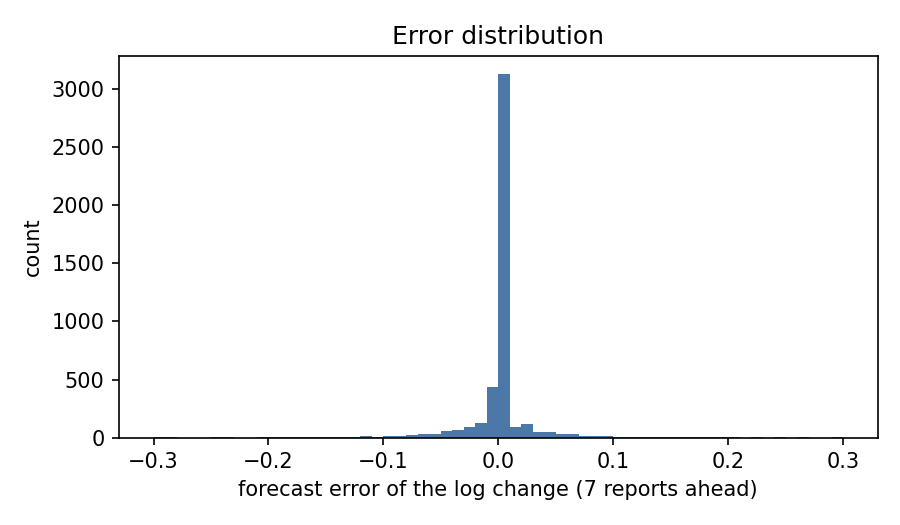
\includegraphics[width=0.7\textwidth]{F11_error_distribution.png}
\caption[Forecast error distribution at horizon 7]{Distribution of the forecast error of the log change, 7 report days ahead (errors clipped at $\pm0.3$).}\label{fig:dist}
\par\smallskip{\footnotesize Source: \path{reports/project/figures/F11}.}
\end{figure}

\begin{figure}[H]
\centering
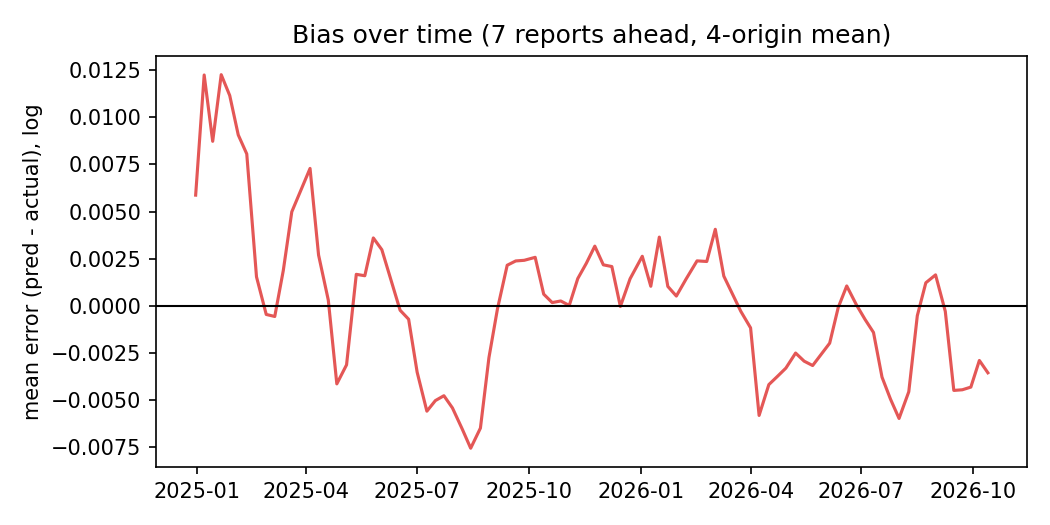
\includegraphics[width=0.75\textwidth]{F12_bias_over_time.png}
\caption[Bias over time at horizon 7 (four-origin mean)]{Bias over time at horizon 7 (four-origin mean).}\label{fig:bias}
\par\smallskip{\footnotesize Source: \path{reports/project/figures/F12}.}
\end{figure}

\begin{figure}[H]
\centering
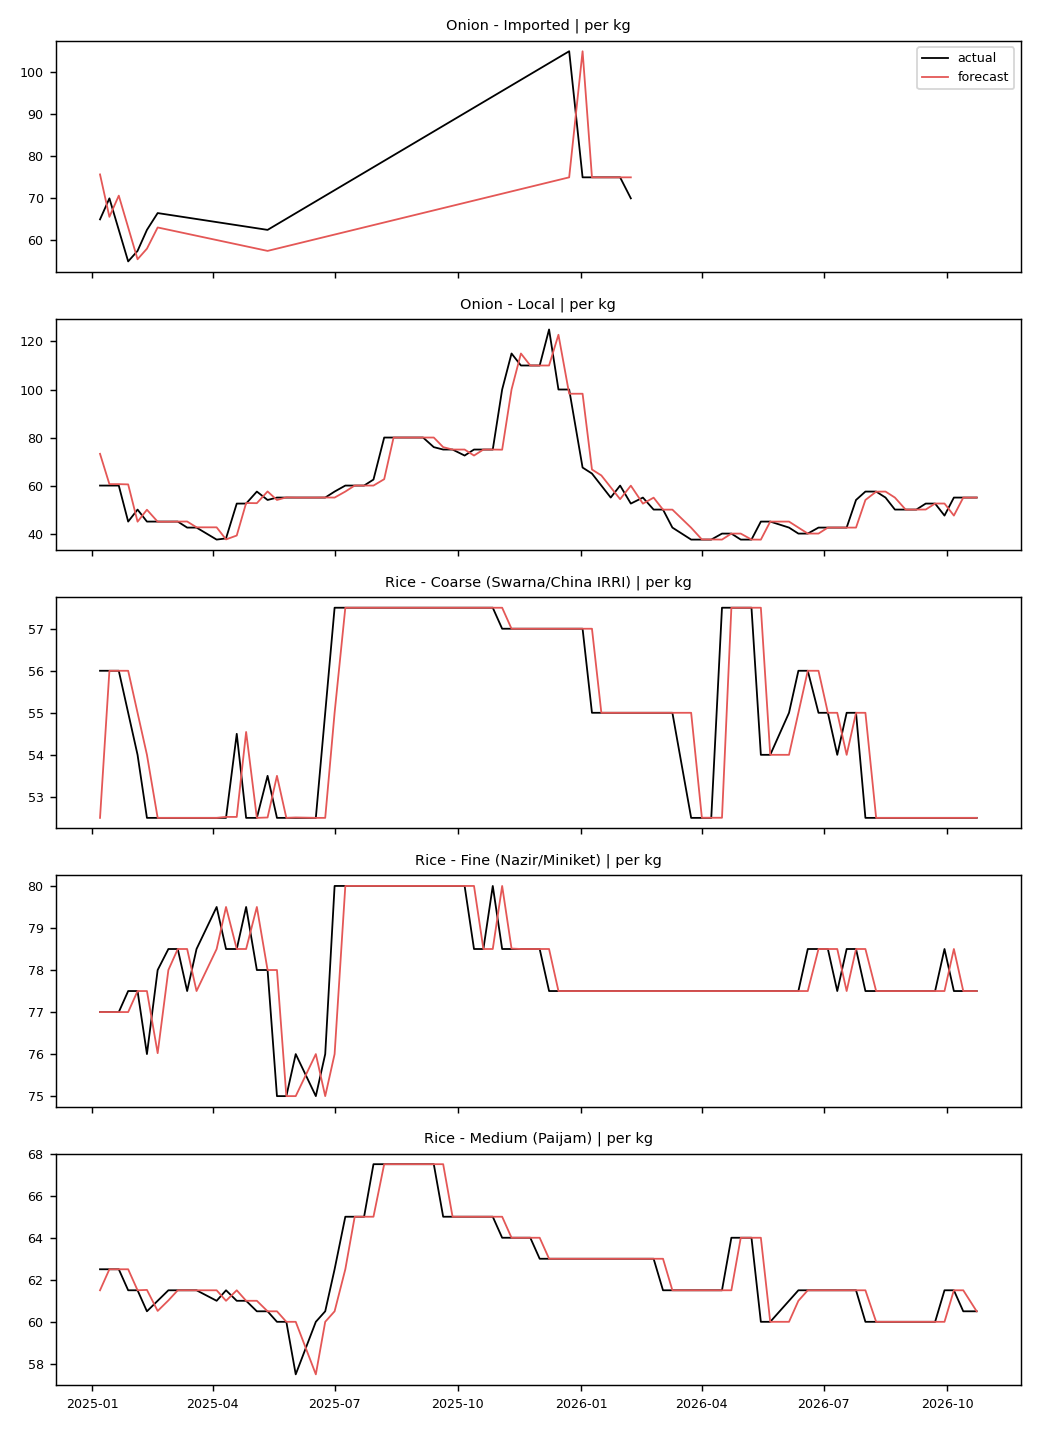
\includegraphics[width=0.85\textwidth]{F14_actual_vs_forecast.png}
\caption[Actual and forecast prices at horizon 7 for five items on the test]{Actual and forecast prices at horizon 7 for five items on the test.}\label{fig:avf}
\par\smallskip{\footnotesize Source: \path{reports/project/figures/F14}.}
\end{figure}

\subsection{Expected Ranges}
At horizon 7, over 55,337 daily forecasts from June 2023 to October 2026, the upper bound at the 0.95 level was exceeded on 5.9\% of days, against 5\% expected, so the upper bound covered 0.941 of the outcomes. The central interval between the 5th and 95th percentiles covered 0.883 against 0.90 expected. The Kupiec test rejects the nominal rate ($p<0.001$), but with this many dependent observations the test is strict, and the practical gap is under one percentage point on the upper side. The result was similar in the two periods (upper coverage 0.939 in 2023--24 and 0.943 in 2025--26), and the bound was narrower in the second period (mean width 0.088 against 0.121 in log terms). The ranges are slightly too tight, not badly so.

\subsection{Alerts}
Table~\ref{tab:level} shows how the alert level was chosen. At the 0.90 level there were 3.07 false alarms per item-year in 2024 outside the event windows, which is over the target of 2, and 0.95 was the lowest level under it (1.92). Level 0.95 was therefore fixed, and the scoring of the episodes came after that.

\begin{table}[H]\centering\small
\caption[Alert levels and false alarms]{Alert levels. False alarms are alert runs per item-year in 2024 outside event windows; recall and precision are over the whole period, counted by product row.}\label{tab:level}
\begin{tabular}{rrrrr}
\toprule
\textbf{Level} & \textbf{False alarms, 2024} & \textbf{Event recall} & \textbf{Precision} & \textbf{Alert runs} \\
\midrule
0.90 & 3.07 & 0.688 & 0.061 & 635 \\
0.95 (chosen) & 1.92 & 0.688 & 0.061 & 429 \\
0.975 & 1.63 & 0.625 & 0.054 & 368 \\
0.99 & 1.44 & 0.500 & 0.052 & 327 \\
\bottomrule
\end{tabular}

\par\smallskip{\footnotesize Source: \path{reports/project/tables/P8_level_curve.csv}.}
\end{table}

At the chosen level, alerts started inside the window of 7 of the 12 episodes (11 of 16 product rows; Table~\ref{tab:events}). The misses are the sugar episode of June 2023, two potato episodes in 2024, the egg episode of October 2024 and the green chilli episode of July 2026. The negative lead times in the table should not be read as early warning. The windows open 14 days before the recorded onset and can run for months after the news peak (the rice episode runs to June 2025), so an alert that starts anywhere inside counts as a detection. The long windows also help the detection rate, since a single alert run anywhere inside a 600-day window is enough.

The random-date control puts the detection rate in perspective. When each episode's window was moved to a random start inside the evaluation period, the mean recall was 0.59, against 0.69 observed, and 26\% of the random draws did as well or better ($p=0.26$ over 300 draws). So the alerts are not distinguishable from chance on these 12 episodes. Of 429 alert runs, only 6\% (26 runs) began inside an event window; the others were not matched to any of the documented episodes. Some of these may be real rises that were not in the news-based list, but the list is the only reference I have, and the system cannot tell the two cases apart.

\begin{table}[H]\centering\small
\caption[The 12 documented episodes and alert detection]{The 12 documented episodes and whether an alert started inside the window (level 0.95). Lead is the number of days between the first alert and the news peak, negative if before.}\label{tab:events}
\begin{tabular}{llllrr}
\toprule
\textbf{Episode} & \textbf{Product} & \textbf{Onset} & \textbf{News peak} & \textbf{Detected} & \textbf{Lead (days)} \\
\midrule
BD-S09 & Sugar & 2023-06-01 & 2023-06-25 & no & -- \\
BD-S11 & Eggs (farm) & 2023-08-01 & 2023-08-13 & yes & 0 \\
BD-S12 & Onion (imported, local) & 2023-08-01 & 2023-08-21 & yes & $-4$ \\
BD-S13 & Onion (imported, local) & 2023-10-01 & 2023-12-09 & yes & $-38$ \\
BD-S14 & Potato & 2023-10-01 & 2023-11-13 & yes & $-12$ \\
BD-S15 & Rice (coarse, medium) & 2023-10-01 & 2025-06-10 & yes & $-558$ \\
BD-S16 & Eggs (farm) & 2024-05-01 & 2024-05-19 & yes & $-11$ \\
BD-S17 & Potato & 2024-07-01 & 2024-08-18 & no & -- \\
BD-S19 & Potato & 2024-09-01 & 2024-09-05 & no & -- \\
BD-S20 & Eggs (farm) & 2024-10-01 & 2024-10-18 & no & -- \\
BD-S21 & Soybean oil (bottled, loose) & 2024-10-01 & 2025-02-09 & yes & $-125$ \\
BD-S22 & Green chilli & 2026-07-01 & 2026-07-31 & no & -- \\
\bottomrule
\end{tabular}

\par\smallskip{\footnotesize Source: \path{reports/project/tables/P8_event_scores.csv}.}
\end{table}

\subsection{Driver Breakdown}
On the last 120 report days, price history accounts for 56\% of the average size of the model's contributions, the exchange rate for 17\%, the calendar for 14\%, the onion export measure for 10\% and weather for 4\% (Table~\ref{tab:drivers}). Because the model forecasts nearly zero change, these are shares of small numbers. They describe what the model leans on, not how much a driver moved a price. The shares look similar across item groups, with price history at 46\% to 68\% in every group, and the exchange rate larger for non-food items and spices (about 24\% and 22\%).

\begin{table}[H]\centering\small
\caption[Driver group shares, last 120 report days]{Share of the average absolute contribution by driver group, last 120 report days.}\label{tab:drivers}
\begin{tabular}{lrrrr}
\toprule
\textbf{Group} & \textbf{Final model} & \textbf{Fitted to day 1211} & \textbf{Fitted to day 1011} & \textbf{Spread} \\
\midrule
Price history & 0.556 & 0.359 & 0.241 & 0.315 \\
Exchange rate & 0.170 & 0.017 & 0.102 & 0.153 \\
Calendar & 0.138 & 0.009 & 0.122 & 0.130 \\
Onion export measure & 0.096 & 0.008 & 0.067 & 0.088 \\
Weather & 0.040 & 0.607 & 0.468 & 0.567 \\
\bottomrule
\end{tabular}

\par\smallskip{\footnotesize Source: \path{reports/project/tables/P9_driver_overall.csv} and \path{P9_driver_stability.csv}.}
\end{table}

The breakdown is not stable. The model fitted to data up to report day 1211 gave weather 61\% and price history 36\%, and the model fitted to day 1011 gave weather 47\%. The final model gives weather 4\%. A tool that moves this much between refits cannot be used to say what drives a price, and I describe the drivers as helpful for specific items, not proven. Two sign checks were planned. The price-above-recent-mean input has the expected sign (correlation $-0.18$ with its contribution, meaning a price high against its recent mean pulls the forecast down). The exchange-rate check returned no value and I did not find out why in the time available. At horizons 1 and 7 the shares are identical to many decimals, which fits a model whose trees never split between those two horizons, in line with the finding that it forecasts almost no change.

\section{Sample Input and Output}

\subsection{Input}
The input is the price file up to the last report day, 24 October 2026, and the driver files. For a given item the model uses the last reported price, its recent changes and volatility, the calendar position and, where the item has them, weather and the exchange rate.

\subsection{Forecast and Range}
For broiler chicken the last reported price was 185 Tk. The 1-report-day forecast was 185 Tk with a range from 179.4 to 190.4 Tk. For small cardamom, last price 5,100 Tk, the 1-report-day forecast was 5,100 Tk with a range from 5,099.3 to 5,135.9 Tk. For the loose atta price of 50 Tk the range at horizon 1 collapses to a single value, 50 Tk. These are rows of the production export, which holds 216 forecasts (54 items at four horizons).

\subsection{Alert and Driver Breakdown}
For each alert day the export file lists the contribution of each driver group, the expected change, and the part of the rise above the upper bound with the note that it is \unexpl. There are 429 alert runs and 3,081 alert days in the export. The note describes the model's inputs only; it does not say that anyone caused a rise.

\subsection{Dashboard}
A local Streamlit dashboard and a Gradio app in Colab read the three export files. They show the forecast and range for a chosen item, the recent alerts, and the driver chart for an alert day. Both state on the first screen that the alerts are not an early warning and that the model did not beat ``tomorrow equals today'' on the test.

\section{Discussion}
The main result is that the forecasts add nothing to persistence on these data. The prices change on few days, the model's best move is to predict no change, and the inputs I could measure did not predict the days when a price does change. The ETS and LightGBM results on 2024 and the walk-forward checks point the same way, and the learning curve shows the model has little to learn from its inputs. This agrees with the AgriPriceBD benchmark, where naive persistence was best for four of five commodities \cite{agripricebd}, so it is not a flaw of one model.

The ranges are usable as an expected band, since the upper bound is exceeded close to the nominal rate, but they are narrow because the model forecasts little movement. The alerts are weaker than the ranges suggest. The detection rate of 7 of 12 episodes is no better than random dates, only 6\% of alert runs lie inside a documented episode, and the long episode windows make detection easy. The system can flag unusual rises for a person to look at; it cannot yet say which flagged rises matter. The driver breakdown is the least reliable part, because its shares change a great deal when the model is refitted.

What can be relied on is the process: the settings were fixed before the test, the test was scored once, a rerun reproduced the same numbers, and every number in this report is listed in a results register with its file and command.
